\section{RQ08 (bônus): rework rate}
\label{sec:rq08}
% Gerado por analises.sprint3_c; não edite à mão.
\newcommand{\labCReworkN}{289}
\newcommand{\labCReworkAusentes}{11}
\newcommand{\labCReworkMediana}{37,3}
\newcommand{\labCReworkTotal}{11.453}
\newcommand{\labCReworkCorretivas}{3.673}
\newcommand{\labCReworkSemEvidencia}{1.899}
\newcommand{\labCReworkLimInf}{32,07}
\newcommand{\labCReworkLimSup}{48,65}
\newcommand{\labCReworkConservadorN}{201}
\newcommand{\labCReworkConservadorMediana}{40,0}
\newcommand{\labCReworkPareados}{289}
\newcommand{\labCReworkDifMediana}{11,1}
\newcommand{\labCReworkMaior}{178}
\newcommand{\labCCUmCDoisN}{269}
\newcommand{\labCCUmCDoisMudou}{39,4}
\newcommand{\labCCUmCDoisKappa}{0,455}
\newcommand{\labCCUmCTresN}{269}
\newcommand{\labCCUmCTresMudou}{40,1}
\newcommand{\labCCUmCTresKappa}{0,437}
\newcommand{\labCCDoisCTresN}{269}
\newcommand{\labCCDoisCTresMudou}{4,5}
\newcommand{\labCCDoisCTresKappa}{0,931}


\textbf{Definição e método.} Escolhemos a opção de \textit{rework rate}: número de
releases principais corretivas dividido pelo total de releases principais publicadas
na janela, por projeto. Reutilizamos a heurística v3 e as regras de disponibilidade
da RQ03~(b), sem recalibrá-las nesta análise. Drafts e pré-releases ficam fora; os
últimos sete dias permanecem no denominador, pois identificar uma corretiva não exige
observar uma release posterior. Releases e commits vêm das fontes congeladas da S02,
com hashes conferidos; o CFR~(b) recalculado deve reproduzir o dataset nos 300 projetos.
Esta análise bônus é descritiva, sem uma nova hipótese retrospectivamente registrada.

\begin{table}[htbp]
\centering\footnotesize
\caption{RQ08: taxas por projeto. A sensibilidade de evidência completa não substitui
a definição principal; quartis usam apenas os casos disponíveis em cada linha.}
\label{tab:rq08}
% Gerado por analises.sprint3_c; não edite à mão.
\begin{tabular}{lrrrr}
\hline
Indicador & $n$ & Ausentes & Mediana (\%) & Q1--Q3 (\%) \\
\hline
Rework rate & 289 & 11 & 37,3 & 20,0--57,1 \\
CFR (b) & 289 & 11 & 17,5 & 0,0--42,9 \\
Rework (evidência completa) & 201 & 99 & 40,0 & 21,4--58,3 \\
\hline
\end{tabular}

\end{table}

\textbf{Resultados.} O rework rate mediano é \labCReworkMediana\%, disponível para
\labCReworkN\ projetos; \labCReworkAusentes\ ficam ausentes pelas regras da S02, sem
imputação por zero. Nos mesmos \labCReworkPareados\ projetos, o rework supera o
CFR~(b) em \labCReworkMaior\ casos; a diferença pareada mediana é
\labCReworkDifMediana\ pontos percentuais. A Figura~\ref{fig:rq08} permite comparar
as distribuições e cada par, sem atribuir causalidade à diferença.

\begin{figure}[htbp]
\centering
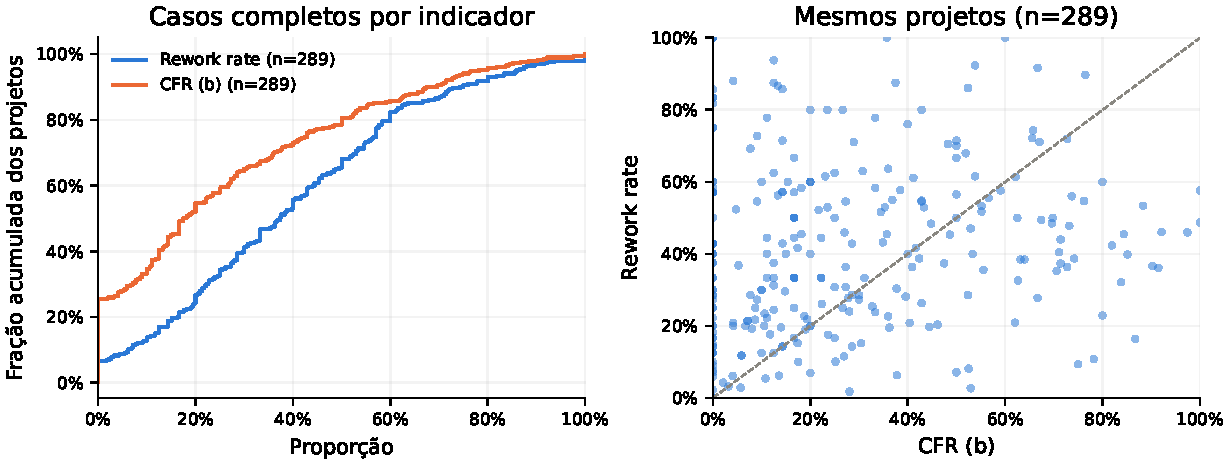
\includegraphics[width=\textwidth]{../../results/s03_c/rq08_rework_cfr.pdf}
\caption{RQ08: distribuição acumulada das taxas e comparação no mesmo projeto.
A diagonal representa igualdade; cada projeto tem o mesmo peso.}
\label{fig:rq08}
\end{figure}

\textbf{Diferença em relação ao CFR~(b).} Rework conta a própria release corretiva,
independentemente de quanto tempo decorreu desde a anterior. CFR~(b) conta releases
anteriores seguidas de uma corretiva em até sete dias e censura os últimos sete dias
da janela. Uma única corretiva pode marcar várias releases anteriores como falhas,
mas entra uma única vez no numerador de rework. Por exemplo, quatro releases em dias
consecutivos, somente a última corretiva, produzem rework de 25\% e CFR~(b) de 75\%,
fora da fronteira censurada. Nenhuma relação de ordem entre as duas taxas é garantida.

\textbf{Sensibilidade e limites.} A regra herdada pode classificar como não corretiva
uma release sem antecessora ou sem commits comparáveis; mensagens incompletas também
podem alterar o balanço entre correções e funcionalidades. Por isso, uma análise
separada trata como desconhecida qualquer release sem comparação bem-sucedida, ao
menos um commit e todas as mensagens preenchidas. São \labCReworkSemEvidencia\ de
\labCReworkTotal\ releases sem essa evidência completa. Restam
\labCReworkConservadorN\ projetos completamente observáveis, com mediana de
\labCReworkConservadorMediana\%. No conjunto das releases, atribuir a todas as
desconhecidas rótulos negativos ou positivos delimita a proporção entre
\labCReworkLimInf\% e \labCReworkLimSup\%. Esses limites não são intervalos de
confiança nem uma média das taxas por projeto; tampouco corrigem erros da heurística.

O DORA define \textit{deployment rework rate} em termos de implantações não planejadas
decorrentes de incidentes em produção~\cite{doraMetricas}. Nosso indicador operacional,
solicitado pelo enunciado, usa releases corretivas como proxy: o GitHub não comprova
que foram implantações, não planejadas ou motivadas por incidentes. Assim, a análise
responde à RQ08 sem equiparar esse proxy à medida operacional do DORA.
